% !TeX spellcheck = <none>
%%%%%%%%%%%%%%%%%%%%%%%%%%%%%%%%%%%%%%%%%
% Beamer Presentation
% LaTeX Template
% Version 1.0 (10/11/12)
%
% This template has been downloaded from:
% http://www.LaTeXTemplates.com
%
% License:
% CC BY-NC-SA 3.0 (http://creativecommons.org/licenses/by-nc-sa/3.0/)
%
%%%%%%%%%%%%%%%%%%%%%%%%%%%%%%%%%%%%%%%%%

%----------------------------------------------------------------------------------------
%	PACKAGES AND THEMES
%----------------------------------------------------------------------------------------

\documentclass{beamer}

\mode<presentation> {

\usetheme{Madrid}

\graphicspath{{./images/}} 



}

\usepackage{graphicx} % Allows including images
\usepackage{booktabs}
\usepackage[T1]{fontenc}
\usepackage[utf8]{inputenc}
\usepackage[english,brazil]{babel} % Allows the use of \toprule, \midrule and \bottomrule in tables

\usepackage{listings}
\usepackage{color}

\definecolor{dkgreen}{rgb}{0,0.6,0}
\definecolor{gray}{rgb}{0.5,0.5,0.5}
\definecolor{mauve}{rgb}{0.58,0,0.82}

\lstset{
	language=Java,
	aboveskip=2mm,
	belowskip=2mm,
	showstringspaces=false,
	columns=flexible,
	basicstyle={\small\ttfamily},
	numbers=none,
	numberstyle=\tiny\color{gray},
	keywordstyle=\color{blue},
	commentstyle=\color{dkgreen},
	stringstyle=\color{mauve},
	breaklines=false,
	breakatwhitespace=true,
	tabsize=1
}

%----------------------------------------------------------------------------------------
%	TITLE PAGE
%----------------------------------------------------------------------------------------

\title[TDD com Android]{Introdução A Testes de Unidade em Aplicativos Android} 
\author{Fernando Avanzo} % Your name
\institute[] 
{ % Your institution for the title page
\medskip
\textit{fernando.avanzo@gmail.com} % Your email address
}
\date{\today} % Date, can be changed to a custom date

\begin{document}

\begin{frame}
\titlepage % Print the title page as the first slide
\end{frame}

\begin{frame}
\frametitle{Overview} 
\tableofcontents % Throughout your presentation, if you choose to use \section{} and \subsection{} commands, these will automatically be printed on this slide as an overview of your presentation
\end{frame}

%----------------------------------------------------------------------------------------
%	PRESENTATION SLIDES
%----------------------------------------------------------------------------------------

%------------------------------------------------
\section{Intro} % Sections can be created in order to organize your presentation into discrete blocks, all sections and subsections are automatically printed in the table of contents as an overview of the talk
%------------------------------------------------

\subsection{Tdd com Android} % A subsection can be created just before a set of slides with a common theme to further break down your presentation into chunks

%------------------------------------------------
\begin{frame}
\frametitle{O que é TDD?}
TDD,(Test Drive Development), é uma prática de desenvolvimento de software que orienta a antes de escrever qualquer código funcional, escrever um coódigo de teste, em seguida escrever o minimo de codigo funcional que faça o teste passar. Então trabalhar esse fluxo de forma incremental em todo o durante todo o processe de desenvolvimento.
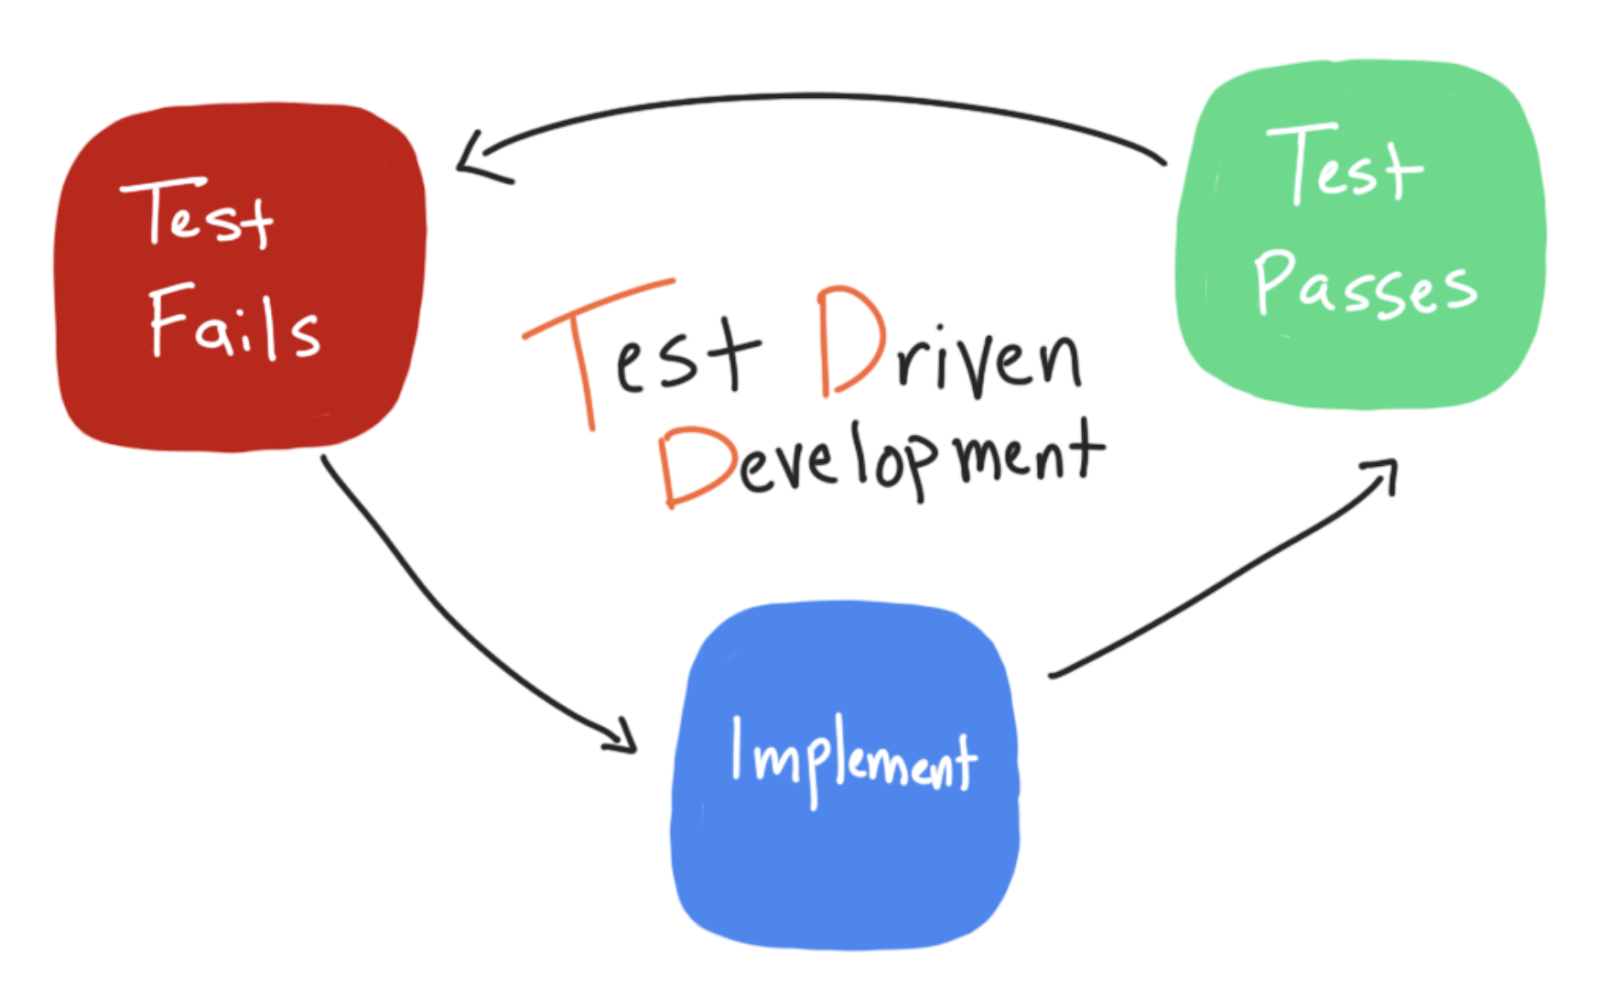
\includegraphics[scale=0.15]{tdd_diagram_flow}
 
\end{frame}

%------------------------------------------------
\begin{frame}
	\frametitle{O Jeito de Pensar TDD}
	Um teste de unidade pode ser escrito em três etapas:
	\begin{block}{Dado (Given)}
		Qual é o estado atual? Nesta etapa os dados necessarios para simular o estado atual da aplicação é fornecido.
	\end{block}
	
	\begin{block}{Quando (When)}
		Quando o estado muda? Nesta etapa o trecho de código, (método, função, procedimento, etc..), que muda o estado é executado.
	\end{block}
	
	\begin{block}{Então (Then)}
		A resposta,(saída), esta certa? Nesta etapa é verificado se após o estado inicial ter sido alterado o resultado corresponde ao esperado.
	\end{block}
	
\end{frame}

%------------------------------------------------
\begin{frame}
	\frametitle{Caso de Uso: ToDo App}
	Vamos ver um exemplo pratico da abordagem GWT, (Given, When, Then) com o aplicativo ToDo
	\begin{columns}[c]
		
		\column{0.1\textwidth} % Left column and width
		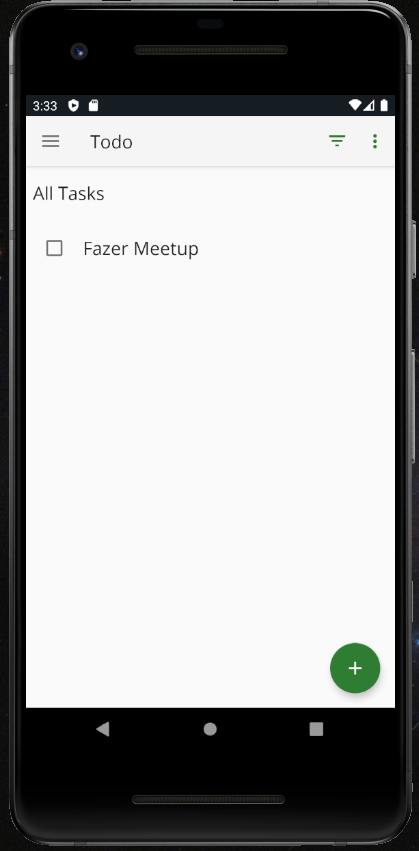
\includegraphics[scale=0.3]{toDoAppSample}
		\column{0.3\textwidth} % Right column and width
		Classico aplicativo de lista tarefas, que permite que usuario adicione uma nova tarefa na lista, check aquelas que já foram concluidas, e veja uma estatistica simples de quantas atividades ele ja conclui, e quantas ainda possui na lista.
		
	\end{columns}
	
\end{frame}

%---------------------------------------------------------------------------------------
\begin{frame}
\frametitle{Caso de Uso: ToDo App}
Cenario de uso: O usuario tem uma lista de tarefas
\begin{itemize}
\item \textbf{Dado} que usuario possui uma lista de tarefas
\item \textbf{Quando} a lista de tarefas conter apenas uma tarefa, e ela estiver completa.
\item \textbf{Então} a porcentagem de tarefas ativas deve ser 0, e porcentagem de tarefas concluidas deve ser 100
\end{itemize}
\end{frame}
%-----------------------------------------------------------------------------------------

%---------------------------------------------------------------------------------------
\begin{frame}[fragile]
	\frametitle{Caso de Uso: ToDo App}
	\begin{example}[Escrevendo o teste]
		\begin{lstlisting}
		@Test
		fun getActiveAndCompletedStats_noActive_returnsZeroHundred() {
			//Given
			val tasks = listOf(Task("title", "desc", isCompleted = true))
			
			// When 
			val result = getActiveAndCompletedStats(tasks)
		
			// Then 
			assertThat(result.activeTasksPercent, `is`(0f))
			assertThat(result.completedTasksPercent, `is`(100f))
		}
		\end{lstlisting}
	\end{example}
\end{frame}
%-----------------------------------------------------------------------------------------

%---------------------------------------------------------------------------------------
\begin{frame}[fragile]
	\frametitle{Caso de Uso: ToDo App}
	\begin{example}[Escrevendo o codigo funcional]
		\begin{lstlisting}
		internal fun getActiveAndCompletedStats(tasks: List<Task>?)
		: StatsResult {
		
			val totalTasks = tasks!!.size
			val numberOfActiveTasks = tasks.count { it.isActive }
			val activePercent = 100 * numberOfActiveTasks / totalTasks
			val completePercent = 100 * (totalTasks - numberOfActiveTasks) / totalTasks
		
			return StatsResult(
				activeTasksPercent = activePercent.toFloat(),
				completedTasksPercent = completePercent.toFloat())
		}
		\end{lstlisting}
	\end{example}
\end{frame}
%-----------------------------------------------------------------------------------------

%---------------------------------------------------------------------------------------
\begin{frame}
	\frametitle{Caso de Uso: ToDo App}
	Cenario de Bug: Temos uma lista com elemento nulo
	\begin{itemize}
		\item \textbf{Dado} que uma lista com elemento nulo
		\item \textbf{Quando} a lista de tarefas conter apenas uma tarefa, e ela for nula.
		\item \textbf{Então} a porcentagem de tarefas ativas e concluidas deve ser 0
	\end{itemize}
\end{frame}
%-----------------------------------------------------------------------------------------


\begin{frame}
\frametitle{Figure}
Uncomment the code on this slide to include your own image from the same directory as the template .TeX file.
%\begin{figure}
%\includegraphics[width=0.8\linewidth]{test}
%\end{figure}
\end{frame}

%------------------------------------------------

\begin{frame}[fragile] % Need to use the fragile option when verbatim is used in the slide
\frametitle{Citation}
An example of the \verb|\cite| command to cite within the presentation:\\~

This statement requires citation \cite{p1}.
\end{frame}

%------------------------------------------------

\begin{frame}
\frametitle{References}
\footnotesize{
\begin{thebibliography}{99} % Beamer does not support BibTeX so references must be inserted manually as below
\bibitem[Smith, 2012]{p1} John Smith (2012)
\newblock Title of the publication
\newblock \emph{Journal Name} 12(3), 45 -- 678.
\end{thebibliography}
}
\end{frame}

%------------------------------------------------

\begin{frame}
\Huge{\centerline{The End}}
\end{frame}

%----------------------------------------------------------------------------------------

\end{document} 